\documentclass[12pt,a4paper]{article}

\usepackage{ctex}   				% 提供中文支持,包括中文文档的字体、字号、标点、章节标题等
\usepackage[colorlinks=false]{hyperref}		% 处理超链接,包括文档内的交叉引用和文献引用,以及生成PDF文档时的超链接,可选参数关闭了超链接的颜色
\usepackage{times}					% 设置文档使用Times字体
\usepackage{amsmath}				% 提供了许多数学排版的增强功能包含了丰富的数学环境、数学命令和数学符号以及众多用于排版数学公式的命令
\usepackage{amsfonts}				% 提供了额外的数学字体如黑板粗体、花体字母
\usepackage{yhmath}					% 使得根号斜率随大小渐变,能适配的尖角括号,\textgoth{}生成哥特字体等
\usepackage{amssymb}				% 包含了许多额外的数学符号,如各种箭头、集合运算符、关系符号等
\usepackage{mathrsfs}				% 提供了一种额外的花体字母
\usepackage{graphicx}				% 用于插入和处理图形
\usepackage{subcaption}				% 允许在一个浮动体中包含多个子图
\usepackage{float}					% 提供浮动体的控制
\usepackage{adjustbox}				% 提供图形和表格的调整选项
\usepackage{bibentry}				% 提供\bibentry{key}命令,可以在文档中嵌入引用文献的完整内容,允许在文档正文中显示完整的文献条目,而不是仅在参考文献列表中显示
\usepackage[numbers]{natbib}		% 提供了更强大和灵活的文献引用功能,支持多种引用风格
\usepackage{abstract}				% 用于定制摘要的格式
\usepackage{xcolor}					% 提供颜色相关的命令和选项
\usepackage{url}					% 提供了处理超链接和网址的命令,支持在文档中插入可点击的链接
\usepackage{bm}						% 允许在数学模式中使用\bm命令给符号加粗
\usepackage{multirow}				% 用于在表格中合并多行
\usepackage{booktabs}				% 用于改进表格的横线显示,提供了更美观的水平线风格
\usepackage{epstopdf}				% epstopdf 将 EPS 转换为PDF格式
\usepackage{epsfig}					% epsfig 提供了在文档中插入EPS图形的命令。
\usepackage{longtable}				% 提供了 longtable 环境,该环境允许表格在页面之间分页,保证表头和表尾在每一页都能正确显示
\usepackage{supertabular}			% 提供了 supertabular 环境,类似于 longtable,允许表格在页面之间分页,但 supertabular 具有更多的自定义选项
\usepackage{algorithm}				% 提供了 algorithm 环境,用于排版算法。允许用户在文档中创建算法块,并提供了一些用于控制算法格式和样式的选项。
\usepackage{algorithmic}			% 提供了一系列用于排版伪代码的命令,允许用户使用伪代码描述算法的执行步骤,提供了类似于if, while, for等关键字的命令。
\usepackage{changepage}				% 允许用户使用伪代码描述算法的执行步骤,提供了类似于 if, while, for 等关键字的命令。
\usepackage{enumerate}				% 允许用户自定义列表项的标签和格式
\usepackage{caption}				% 允许用户设置图表标题的格式和样式
\usepackage{indentfirst}			% 让每个章节的第一个段落首行缩进,符合中文排版习惯
\usepackage[left=2.50cm,right=2.50cm,top=2.80cm,bottom=2.50cm]{geometry}	% 提供了设置文档页边距、纸张大小等的命令
\usepackage{fancyhdr}				% 允许用户自定义页眉和页脚的内容、样式和位置
\usepackage{caption}				% 提供了更多的选项,允许用户自定义图表标题的字体、大小、对齐方式等
\usepackage{lipsum}					% 自动生成虚拟文本
\usepackage{multicol}				% 允许在文档中创建多列布局
\usepackage{lettrine}				% 用于创建大型首字母(drop cap)
\usepackage{esint}					% 提供了更多的积分符号
\usepackage{tikz}					% 用于创建图形和绘制矢量图
\usepackage{pgfplots}				% 基于TikZ,专门用于绘制二维和三维的数据图
\usepackage{tikz-3dplot}			% 用于在TikZ中简化三维坐标系的创建和绘制

%%%%%%%%%%%%%%%%%%%%%%%%%%%%%%%%%%%%%%%%%%%%%%%%%%%%%%%%

\pagestyle{fancy}
\hypersetup{colorlinks=false,linkbordercolor=white,allcolors=white,citebordercolor=white,runcolor=white,allcolors=white,filecolor=white,linkcolor=white}
\captionsetup[figure]{name=\fontsize{10pt}{15pt}\selectfont Figure} 
\captionsetup[table]{name=\fontsize{10pt}{15pt}\selectfont Table} 

%%%%%%%%%%%%%%%%%%%%%%%%%%%%%%%%%%%%%%%%%%%%%%%%%%%%%%%%

\renewcommand{\abstracttextfont}{\fangsong} 
\renewcommand{\abstractname}{\textbf{摘\quad 要}} 
\renewcommand{\baselinestretch}{1.5}

\newcommand{\red}[1]{\textcolor[rgb]{1.00,0.00,0.00}{#1}}
\newcommand{\blue}[1]{\textcolor[rgb]{0.00,0.00,1.00}{#1}}
\newcommand{\green}[1]{\textcolor[rgb]{0.00,1.00,0.00}{#1}}
\newcommand{\darkblue}[1]{\textcolor[rgb]{0.00,0.00,0.50}{#1}}
\newcommand{\darkgreen}[1]{\textcolor[rgb]{0.00,0.37,0.00}{#1}}
\newcommand{\darkred}[1]{\textcolor[rgb]{0.60,0.00,0.00}{#1}}
\newcommand{\brown}[1]{\textcolor[rgb]{0.50,0.30,0.00}{#1}}
\newcommand{\purple}[1]{\textcolor[rgb]{0.50,0.00,0.50}{#1}}

%%%%%%%%%%%%%%%%%%%%%%%%%%%%%%%%%%%%%%%%%%%%%%%%%%%%%%%%

\setlength{\parindent}{0pt}			% 取消自动段首缩进

%%%%%%%%%%%%%%%%%%%%%%%%%%%%%%%%%%%%%%%%%%%%%%%%%%%%%%%%
% 自定义巨型算符

\makeatletter
\DeclareRobustCommand\bigop[1]{%
	\mathop{\vphantom{\sum}\mathpalette\bigop@{#1}}\slimits@
}
\newcommand{\bigop@}[2]{%
	\vcenter{%
		\sbox\z@{$#1\sum$}%
		\hbox{\resizebox{\ifx#1\displaystyle.9\fi\dimexpr\ht\z@+\dp\z@}{!}{$\m@th#2$}}%
	}%
}
\makeatother

\newcommand{\bigK}{\DOTSB\bigop{\mathrm{K}}}

%%%%%%%%%%%%%%%%%%%%%%%%%%%%%%%%%%%%%%%%%%%%%%%%%%%%%%%
% 封面信息

\title{\fontsize{18pt}{27pt}\selectfont{\heiti 第八章作业: 振动}} 
\author{\fontsize{12pt}{18pt}\selectfont {\fangsong  林海轩}\\\fontsize{10.5pt}{15.75pt}\selectfont{\fangsong(复旦大学 物理学系)}} 
\date{}

%%%%%%%%%%%%%%%%%%%%%%%%%%%%%%%%%%%%%%%%%%%%%%%%%%%%%%%%
% 注意这部分代码将全角的逗号句号转换为了半角的逗号句号且半角逗号后面跟了一个空格,要求用xelatex编译,但模板撰写的时候默认用pdflatex,不推荐使用

%\catcode`,=\active
%\newcommand{,}{, }

%\catcode`。=\active
%\newcommand{。}{.}

%\catcode`:=\active
%\newcommand{:}{: }
%%%%%%%%%%%%%%%%%%%%%%%%%%%%%%%%%%%%%%%%%%%%%%%%%%%%%%%%
% 自己编写的命令,用于生成不编号但计入目录的标题

\newcommand{\nonumbersection}[1]{
	\section*{#1}
	\addcontentsline{toc}{section}{#1}
}
\newcommand{\nonumbersubsection}[1]{
	\subsection*{#1}
	\addcontentsline{toc}{subsection}{#1}
}
%%%%%%%%%%%%%%%%%%%%%%%%%%%%%%%%%%%%%%%%%%%%%%%%%%%%%%%%

\begin{document}
	
	\lhead{} 
	\chead{} 
	\rhead{} 
	\lfoot{}
	\cfoot{\thepage} 
	\rfoot{} 
	
	\maketitle
	
	\begin{abstract}
		\fangsong 振动是物理学中一个重要的概念, 广泛应用于各个领域, 从微小的原子振动到宏观的机械振动. 本篇作业将深入探讨振动的基本原理, 特征和应用.
	\end{abstract}
	
	\begin{adjustwidth}{1.06cm}{1.06cm}
		\fontsize{10.5pt}{15.75pt}\selectfont{\heiti{关键词: }\fangsong{振动, 物理学.}}\\
	\end{adjustwidth}
	
	%\begin{center}% 居中处理
		%{\textbf{Abstract}}% 英文摘要
	%\end{center}
	%\begin{adjustwidth}{1.06cm}{1.06cm}% 英文摘要内容
		%\hspace{1.5em}In order to improve my computer and English skills, please allow me to complete this physics homework in English context with \LaTeX, so as to improve my professional level. Sorry for the inconvenience!
	%\end{adjustwidth}
	
	\newpage
	
	\renewcommand{\contentsname}{目录}
	\tableofcontents
	
	\newpage
	
%%%%%%%%%%%%%%%%%%%%%%%%%%%%%%%%%%%%%%%%%%%%%%%%%%%%%%%%

	\section{题目8-10}
	
	\nonumbersubsection{(1)}
	
		分别对两球受力分析可得:
		
		\begin{equation}
			T=m_2g=m_1\dfrac{v_0^2}{l_0}
		\end{equation}
		
		解得:
		
		$$
		l_0=\dfrac{m_1v_0^2}{m_2g}
		$$
		
	\nonumbersubsection{(2)}
		
		设 $\delta l$ 为偏离平衡位置的线度, 并且是小量. 根据能量守恒定律可以得到:
		
		\begin{equation}
			E=\dfrac{1}{2}(m_1+m_2)\delta\dot{l}^2+m_2g\delta l+\dfrac{1}{2}m_1\left( \dot{\theta}\left( l_0+\delta l\right) \right) ^2
		\end{equation}
		
		径向的冲量不影响角动量守恒, 所以有:
		
		\begin{equation}
			\dot{\theta}l^2=v_0l_0
		\end{equation}
		
		联立方程, 并对联立式进行 Tailor 展开:
		
		\begin{align}
			E&=\dfrac{1}{2}\left( m_1+m_2\right)\delta\dot{l}^2+m_2g\delta l+\dfrac{1}{2}m_1v_0^2\left( 1+\dfrac{\delta l}{l_0}\right)^2 \nonumber
			\\
			&=\dfrac{1}{2}\left( m_1+m_2\right)\delta\dot{l}^2+m_2g\delta l+\dfrac{1}{2}m_1v_0^2\left( 1-2\dfrac{\delta l}{l_0}+3\dfrac{\delta l^2}{l_0^2}+\cdots\right) \nonumber
			\\
			&=\dfrac{1}{2}\left( m_1+m_2\right)\delta \dot{l}^2+\dfrac{1}{2}3m_1\dfrac{v_0^2}{l_0^2}\delta l^2+\cdots 
		\end{align}
		
		与标准简谐运动的能量守恒方程 $E=\dfrac{1}{2}m\dot{x}^2+\dfrac{1}{2}kx^2$ 对比:
		
		\begin{align}
			\mathcal{M}&=m_1+m_2
			\\
			\mathcal{K}&=3m_1\dfrac{v_0^2}{l_0^2}
		\end{align}
		
		其中, $\mathcal{M}$ 和 $\mathcal{K}$ 是系统的等效质量和等效恢复系数. 根据振动方程的解有:
		
		\begin{equation}
			\omega_0=\sqrt{\dfrac{\mathcal{K}}{\mathcal{M}}}=\sqrt{\dfrac{3m_1\dfrac{v_0^2}{l_0^2}}{m_1+m_2}}
		\end{equation}
		
		代入(1)的结果即可得:
		
		$$
		\omega_0=\dfrac{m_2g}{v_0}\sqrt{\dfrac{3}{m_1\left(m_1+m_2 \right) }}
		$$
		
		\section{题目8-12}
		
		\begin{figure}[H]
			\begin{minipage}{0.4\textwidth}
				\centering
				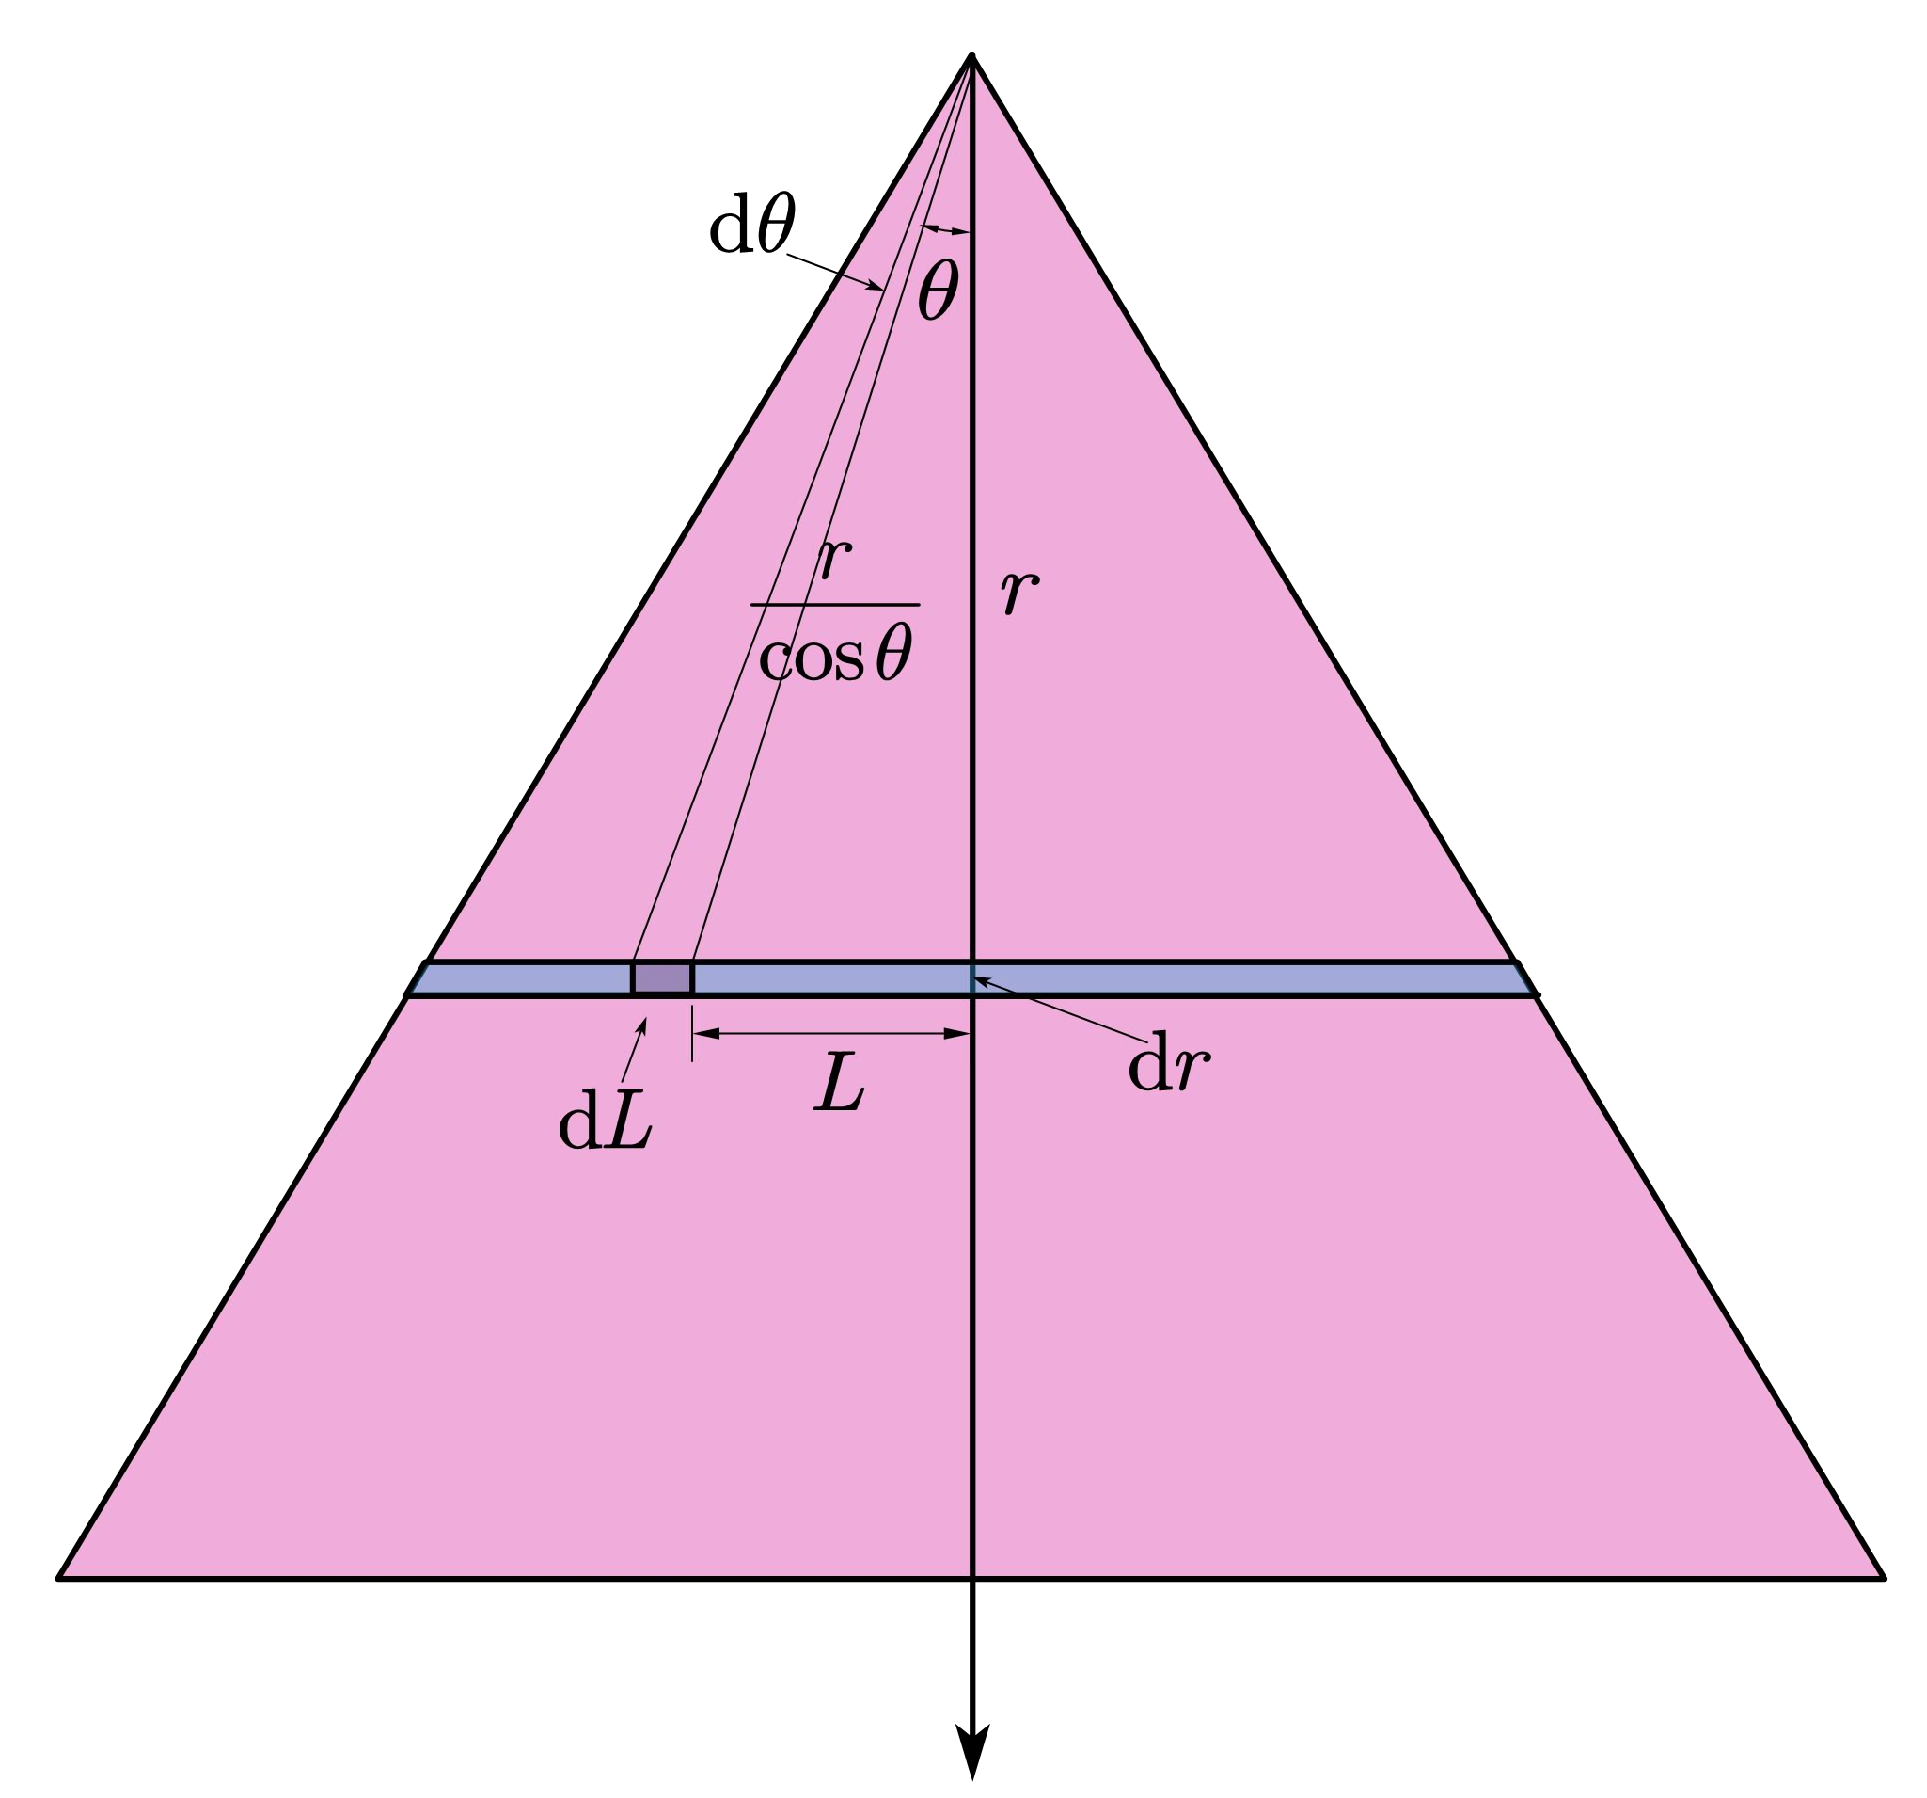
\includegraphics[width=\linewidth]{C:/Users/Administrator/Desktop/VScode/LaTeX/EarlyPic/8-12-2}
				\caption*{}
			\end{minipage}
			\hfill
			\begin{minipage}{0.52\textwidth}
				\centering
				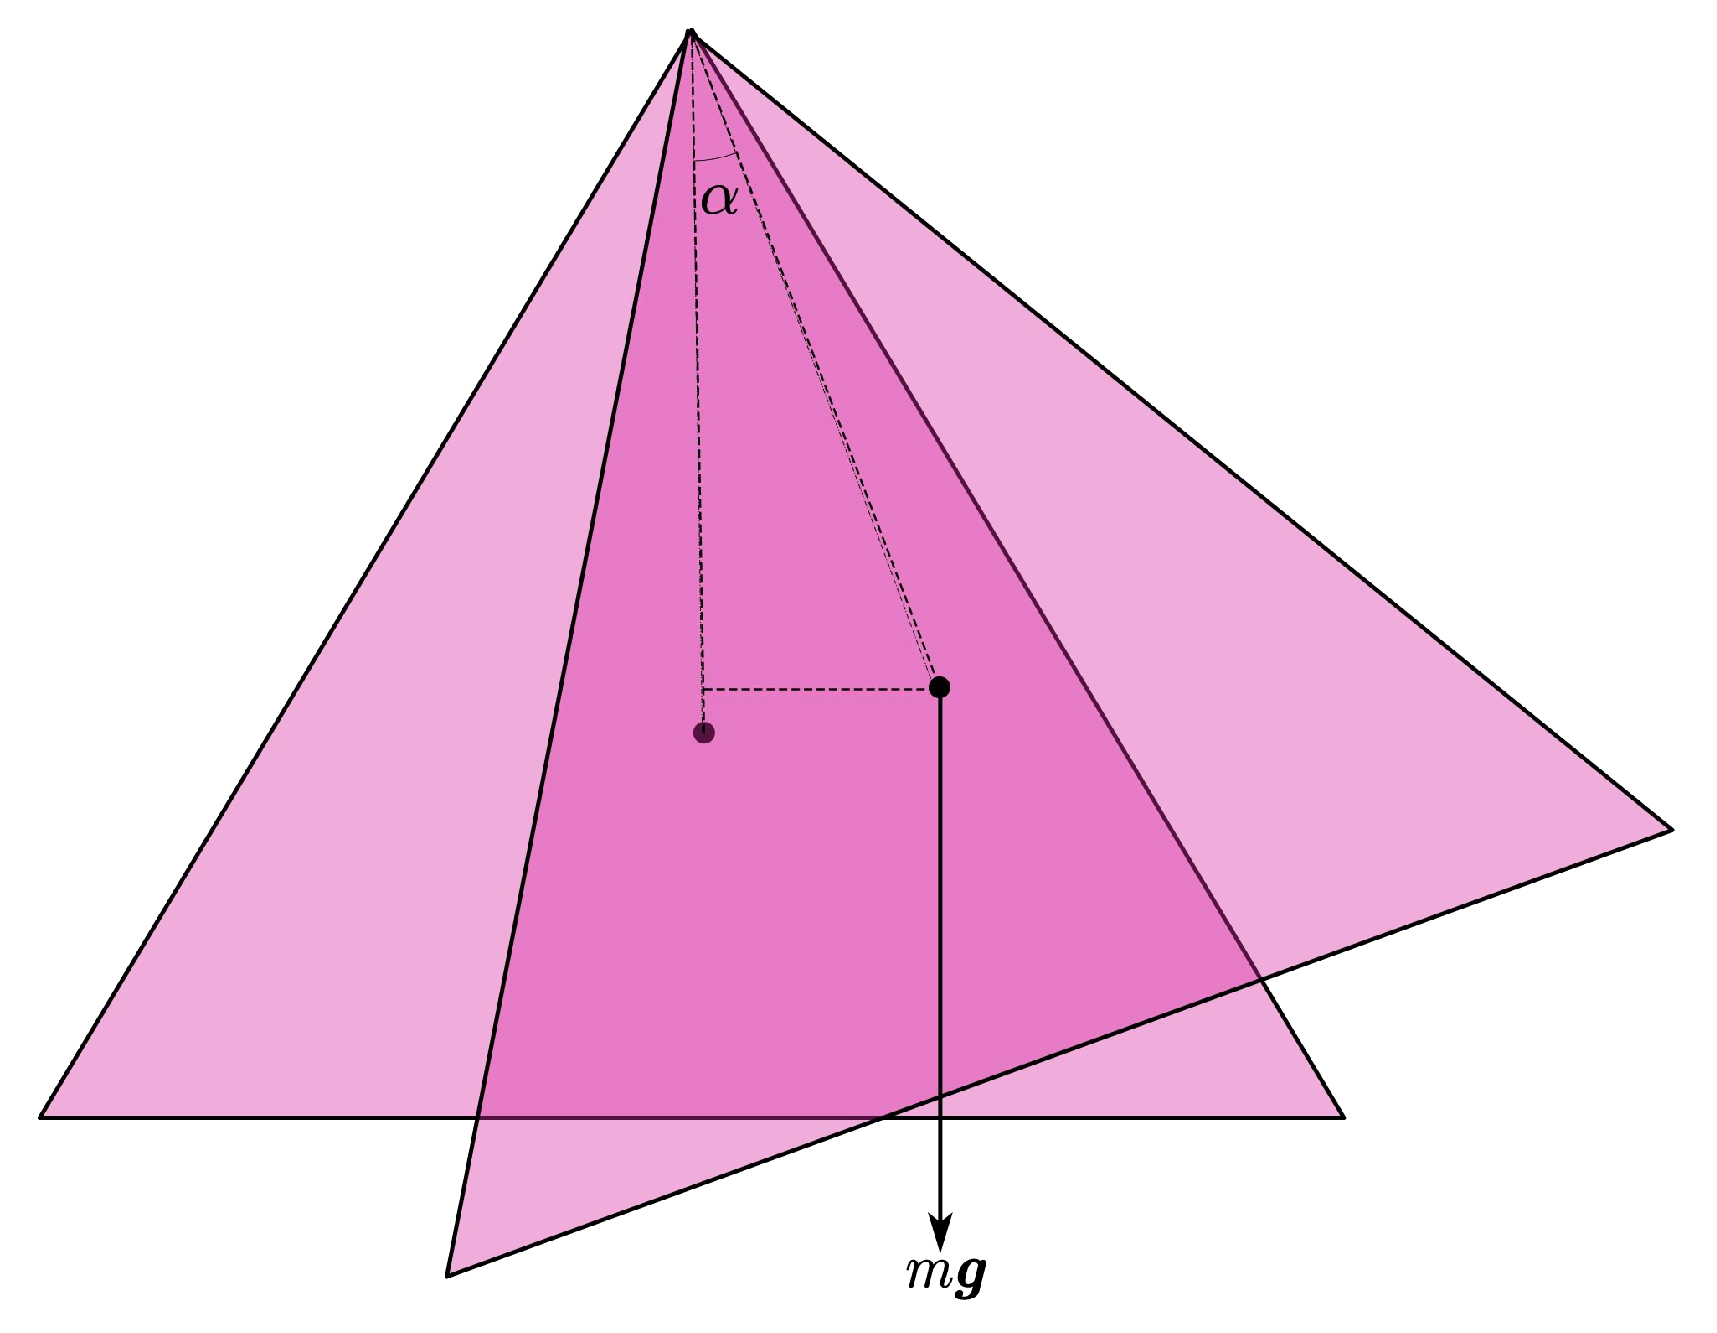
\includegraphics[width=\linewidth]{C:/Users/Administrator/Desktop/VScode/LaTeX/EarlyPic/8-12-1}
				\caption*{}
			\end{minipage}
		\end{figure}
		
		以轴与三角薄板的交点为参考点, 计算三角板定轴转动的转动惯量. 先取一条状微元, 与轴的垂直距离为 $r$, 再在条状微元上取一小段微元, 考究这一小段的转动惯量:
		
		\begin{equation}
			\mathrm{d}J=\mathrm{d}m\dfrac{r^2}{\cos^2\theta }
		\end{equation}
		
		定义面密度: 
		\begin{equation}
			\sigma=\dfrac{m}{S}=\dfrac{m}{\dfrac{\sqrt{3}}{4}a^2}
		\end{equation}
		
		那么有:
		\begin{equation}
			\mathrm{d}m=\dfrac{\mathrm{d}L}{\dfrac{2r}{\sqrt{3}}}\sigma\dfrac{2r}{\sqrt{3}}\mathrm{d}r
		\end{equation}
		
		联立这些方程并积分:
		\begin{equation}
			J=\iint\mathrm{d} J=\int\limits_{0}^{\frac{\sqrt{3}}{2}a}\int\limits_{-\frac{\pi}{6}}^{\frac{\pi}{6}}\dfrac{4m}{\sqrt{3}a^2}\dfrac{r^3}{\cos^4\theta}\mathrm{d}\theta\mathrm{d}r=\dfrac{4m}{\sqrt{3}a^2}\int\limits_{0}^{\frac{\sqrt{3}}{2}a}r^3\mathrm{d}r\int\limits_{-\frac{\pi}{6}}^{\frac{\pi}{6}}\dfrac{\mathrm{d}\theta}{\cos^4\theta}=\dfrac{5}{12}ma^2
		\end{equation}
		
		很容易写出能量守恒方程, 并根据小角度近似做 Tailor 展开:
		\begin{equation}
			E=mg\dfrac{a}{\sqrt{3}}\left( 1-\cos\theta\right)+\dfrac{1}{2}J\dot{\theta}^2 =\dfrac{1}{2}mg\dfrac{a}{\sqrt{3}}\theta^2+\dfrac{1}{2}J\dot{\theta}^2+\cdots
		\end{equation}
		
		与标准简谐运动的能量守恒方程 $E=\dfrac{1}{2}m\dot{x}^2+\dfrac{1}{2}kx^2$ 对比:
		\begin{align}
			\mathcal{M}&=J
			\\
			\mathcal{K}&=mg\dfrac{a}{\sqrt{3}}
		\end{align}
		
		其中, $\mathcal{M}$ 和 $\mathcal{K}$ 是系统的等效质量和等效恢复系数. 根据振动方程的解有:
		
		$$
		T=2\pi\sqrt{\dfrac{\mathcal{M}}{\mathcal{K}}}=2\pi\sqrt{\dfrac{5a}{4\sqrt{3}g}}
		$$
		
		与标准单摆的周期 $T=2\pi\sqrt{\dfrac{l}{g}}$ 对比, 系统的等效摆长为:
		
		$$
		\mathcal{L}=\dfrac{5a}{4\sqrt{3}}
		$$
		
	\section{题目8-13}
		\nonumbersubsection{(1)}
			根据平行轴定理, 容易求出系统相对转轴的转动惯量:
			\begin{equation}
				J=\dfrac{1}{3}ml^2+\dfrac{1}{2}m_0R^2+m_0l^2
			\end{equation}
			
			写出系统的能量并根据小角度进行 Tailor 展开:
			\begin{equation}
				E=mg\dfrac{1}{2}\left( 1-\cos\theta\right)+m_0 gl\left( 1-\cos\theta\right)+\dfrac{1}{2}J\dot{\theta}^2 =\dfrac{1}{2}\left(mg\dfrac{l}{2}+m_0gl \right)\theta^2+\dfrac{1}{2}J\dot{\theta}^2+\cdots 
			\end{equation}
			
			与标准简谐运动的能量守恒方程 $E=\dfrac{1}{2}m\dot{x}^2+\dfrac{1}{2}kx^2$ 对比:
			\begin{align*}
				\mathcal{M}&=J
				\\
				\mathcal{K}&=mg\dfrac{l}{2}+m_0gl
			\end{align*}
			
			其中, $\mathcal{M}$ 和 $\mathcal{K}$ 是系统的等效质量和等效恢复系数. 根据振动方程的解有:
			$$
			T=2\pi\sqrt{\dfrac{\mathcal{M}}{\mathcal{K}}}=2\pi\sqrt{\dfrac{2\left( m+3m_0\right)l^2+3m_0R^2 }{3\left( m+2m_0\right)gl }}
			$$
			
			与标准单摆的周期 $T=2\pi\sqrt{\dfrac{l}{g}}$ 对比, 系统的等效摆长为:
			$$
			\mathcal{L}=\dfrac{2\left( m+3m_0\right)l^2+3m_0R^2 }{3\left( m+2m_0\right)l }
			$$
		\nonumbersubsection{(2)}
		若相连处的轴是光滑的, 那么圆盘是不会有自转的, 因此转动惯量没有由圆盘自转引起的那一项, 也就是说 $J=\dfrac{1}{3}ml^2+m_0l^2$, 据此写出能量表达式并进行 Tailor 展开:
		
		\begin{equation}
			E =\dfrac{1}{2}\left(mg\dfrac{l}{2}+m_0gl \right)\theta^2+\dfrac{1}{2}\left(\dfrac{1}{3}ml^2+m_0l^2 \right) \dot{\theta}^2+\cdots 
		\end{equation}
		
		与标准简谐运动的能量守恒方程 $E=\dfrac{1}{2}m\dot{x}^2+\dfrac{1}{2}kx^2$ 对比:
		\begin{align*}
			\mathcal{M}&=\dfrac{1}{3}ml^2+m_0l^2
			\\
			\mathcal{K}&=mg\dfrac{l}{2}+m_0gl
		\end{align*}
		
		其中, $\mathcal{M}$ 和 $\mathcal{K}$ 是系统的等效质量和等效恢复系数. 根据振动方程的解有:
		$$
		T=2\pi\sqrt{\dfrac{\mathcal{M}}{\mathcal{K}}}=2\pi\sqrt{\dfrac{2\left( m+3m_0\right)l}{3\left( m+2m_0\right)g }}
		$$
		
		与标准单摆的周期 $T=2\pi\sqrt{\dfrac{l}{g}}$ 对比, 系统的等效摆长为:
		$$
		\mathcal{L}=\dfrac{2\left( m+3m_0\right)l}{3\left( m+2m_0\right)}
		$$
		\section{题目8-14}
		对球受力分析, 根据 Newton 第二定律:
		\begin{equation}
			ma=-mg\sin\theta=-mg\dfrac{x}{R-r}+\cdots
		\end{equation}
		上式已依据小角度进行 Tailor 展开, 并且根据纯滚动有关系:
		\begin{equation}
			\dfrac{2}{5}mr^2\beta=\dfrac{2}{5}mr^2\dfrac{a}{r}=fr
		\end{equation}
		上式已经用到了转动定律. 两式联立:
		\begin{equation}
			a+\dfrac{5}{7}\dfrac{g}{R-r}x=0
		\end{equation}
		与标准得弹簧振子方程 $\ddot{x}+\omega_0^2x=0$ 对比, 得到:
		$$
		T=\dfrac{2\pi}{\omega_0}=\dfrac{2\pi}{\sqrt{\dfrac{5}{7}\dfrac{g}{R-r}}}=2\pi\sqrt{\dfrac{7}{5}\dfrac{R-r}{g}}
		$$
		\section{问题8-19}
		\nonumbersubsection{(1)}
		因为 $k_1<k_2$, 所以平衡时物块向右移动一段距离, 设之为 $\Delta x$, 对于物块, 它是受力平衡的:
		\begin{equation}
			k_1\left(\Delta x_0+\Delta x \right)=k_2\left( \Delta x_0-\Delta x\right)  
		\end{equation}
		代入数据解得:
		$$
		\Delta x=5\ \mathrm{cm}
		$$
		所以左端弹簧的长度为 35 cm, 右端弹簧的长度为 25 cm.
		\nonumbersubsection{(2)}
		设向右为正, 离开平衡位置的距离记为 $x$, 受力分析得:
		\begin{equation}
			m\dfrac{\mathrm{d}^2x}{\mathrm{d}t^2}=-\left( k_1+k_2\right)x 
		\end{equation}
		所以
		$$
		T=2\pi\sqrt{\dfrac{m}{k_1+k_2}}=\pi\ \mathrm{s}\approx3.14\ \mathrm{s}
		$$
		\nonumbersubsection{(3)}
		发生得是完全非弹性碰撞, 能量损失为原来的一半, 又因为弹簧振子的能量正比于振幅的平方, 所以振幅为原来的 $\dfrac{1}{\sqrt{2}}$ 倍.
		$$
		A'=\dfrac{A}{\sqrt{2}}=\dfrac{5}{\sqrt{2}}\ \mathrm{cm}\approx3.54\ \mathrm{cm}
		$$
		振动的周期与能量无关:
		$$
		T=2\pi\sqrt{\dfrac{m+\Delta m}{k_1+k_2}}=\sqrt{2}\pi\ \mathrm{s}\approx4.44\ \mathrm{s}
		$$
		\nonumbersubsection{(4)}
		根据上面的论述, 很容易有:
		$$
		A'=A=5\ \mathrm{cm}
		$$
		$$
		T=2\pi\sqrt{\dfrac{m+\Delta m}{k_1+k_2}}=\sqrt{2}\pi\ \mathrm{s}\approx4.44\ \mathrm{s}
		$$
		
		\section{题目8-20}
		不妨考察一般形式的带阻尼项的振动方程:
		\begin{equation}
			\ddot{x}+2\delta\dot{x}+\omega_0^2x=0
		\end{equation}
		
		这个方程的通解为:
		\begin{equation}
			x=A_0\mathrm{e}^{-\delta t}\cos\left(\sqrt{\omega_0^2-\delta^2}t+\phi_0 \right) 
		\end{equation}
		这个解对应的是欠阻尼的情形, 如果 $\omega_0^2-\delta^2<0$ 则会出现虚数的情况, 此时用 Euler 公式 
		$$
		\cos x=\dfrac{\mathrm{e}^{\mathrm{i}x}+\mathrm{e}^{-\mathrm{i}x}}{2}
		$$
		改写, 再取实部的部分. 根据原题意, 可以得到:
		\begin{equation}
			\boldsymbol{f}=m\boldsymbol{a}_f=-2\mu A\boldsymbol{v}\Longrightarrow\delta=\dfrac{\mu A}{m}
		\end{equation}
		根据周期公式:
		\begin{equation}
			T=\dfrac{2\pi}{\sqrt{\omega_0^2-\delta^2}}
		\end{equation}
		\vspace{0.3em}
		\begin{equation}
			T_0=\dfrac{2\pi}{\omega_0}
		\end{equation}
		解得:
		$$
		T_0=\dfrac{2\pi}{\sqrt{\left(\dfrac{2\pi}{T} \right)^2+\left(\mu S \right)^2  }}
		$$
		\section{题目8-25}
		能量的频率是位移量频率的两倍, 容易写出:
		\begin{equation}
			E=E_0\mathrm{e}^{-2\delta t}
		\end{equation}
		在 $t_0=1\ \mathrm{s}$ 后能量减至一半:
		\begin{equation}
			\dfrac{1}{2}E_0=E_0\mathrm{e}^{-2\delta t_0}
		\end{equation}
		根据品质因数 $Q$ 的定义:
		\begin{equation}
			Q=2\pi\dfrac{\Delta E}{E}=\dfrac{2\pi}{1-\mathrm{e}^{-2\delta T}}
		\end{equation}
		同时有:
		\begin{equation}
			T=\dfrac{2\pi}{f}
		\end{equation}
		根据阻尼振动的解:
		\begin{equation}
			2\pi f=\sqrt{\left( 2\pi f_0\right)^2-\delta^2 }
		\end{equation}
		最终解得:
		$$
		Q=\dfrac{2\pi}{1-{\left( \dfrac{1}{2}\right) }^{\dfrac{1}{\sqrt{\left( t_0f_0\right)^-\left( \dfrac{\ln 2}{4\pi}\right)^2  }}}}\approx2323
		$$
		\section{问题8-27}
		\nonumbersubsection{(1)}
		与标准的带阻尼受迫振动运动学方程对比:
		\begin{equation}
			\ddot{x}+2\delta\dot{x}+\omega_0^2x=F
		\end{equation}
		只需证明受迫项 $F=\dfrac{g}{l}x_2$. 以悬点为参考点, 则单摆可以等效为收阻尼和惯性力的谐振子, 其中, 把惯性力放入受迫的那一项, 即可得到:
		$$
		\dfrac{\mathrm{d}^2x_1}{\mathrm{d}t^2}+2\delta\dfrac{\mathrm{d}x_1}{\mathrm{d}t}+\dfrac{g}{l}x_1=\dfrac{g}{l}x_2
		$$
		一般地, 余弦式受迫振动的通解为:
		$$
			x=A_0\mathrm{e}^{-\delta t}\cos \left( \sqrt{{\omega _0}^2-\delta ^2}t+\varphi _0 \right) +\frac{F_0/m}{\sqrt{\left( \omega ^2-\omega _{0}^{2} \right) ^2+4\delta ^2\omega ^2}}\cos \left( \omega t+\mathrm{arc}\tan \frac{2\delta \omega}{\omega ^2-\omega _{0}^{2}} \right) 
		$$
		代入相关系数即可得到:
		$$
		x=A_0\mathrm{e}^{-\delta t}\cos \left( \sqrt{\dfrac{g}{l}-\delta ^2}t+\varphi _0 \right) +\dfrac{Ag/l}{\sqrt{\left( \omega ^2-\dfrac{g}{l} \right) ^2+4\delta ^2\omega ^2}}\cos \left( \omega t+\mathrm{arc}\tan \dfrac{2\delta \omega}{\omega ^2-\dfrac{g}{l}} \right) 
		$$
		其中, $A_0$ 取决于初始的能量, $\varphi_0$ 取决于初始的相位.
		\nonumbersubsection{(2)}
		令 $t\rightarrow+\infty$, 上式右侧的第一项趋于 $0$, 再使得 $\omega=\sqrt{\dfrac{g}{l}}$, 即达到共振, 则:
		$$
		x=\dfrac{Ag/l}{2\delta\omega}\cos \left( \omega t+\mathrm{arc}\tan \dfrac{2\delta \omega}{\omega ^2-\dfrac{g}{l}} \right) 
		$$
		当不考虑受迫的时候:
		\begin{equation}
			A=A_0\mathrm{e}^{-\delta t}
		\end{equation}
		代入 $t=50T$, 以及 $A=\dfrac{A_0}{\mathrm{e}}$, 考虑到:
		\begin{equation}
			T=\dfrac{2\pi}{\sqrt{\omega_0^2-\delta^2}}
		\end{equation}
		最终:
		$$
		A'=\dfrac{\sqrt{10^4\pi^2+1}}{2}A\approx15.7\ \mathrm{cm}
		$$
		\nonumbersubsection{(3)}
		只需要:
		\begin{equation}
			4\delta \sqrt{\dfrac{g}{l}}=\sqrt{\left( \omega ^2-\dfrac{g}{l} \right) ^2+4\delta ^2\omega ^2}
		\end{equation}
		解得:
		$$
		\omega =\sqrt{\frac{g}{l}-2\delta ^2\pm \sqrt{4\delta ^2+12\frac{g}{l}\delta ^2}}=3.147\ \mathrm{rad/s}, 3.113\ \mathrm{rad/s}
		$$
		\section{题目8-34}
		\nonumbersubsection{(1)}
		同频时候振幅为同向线性叠加, 所以
		$$
		\varphi_2=\dfrac{\pi}{6}+2k\pi
		$$
		$$
		A=A_1+A_2=0.6\ \mathrm{m}
		$$
		其中, $k\in\mathbb{Z}$.
		\nonumbersubsection{(2)}
		根据初相位公式得到:
		\begin{equation}
			\varphi=\arctan\dfrac{A_1\sin\varphi_1+A_2\sin\varphi_2}{A_1\cos\varphi_1+A_2\cos\varphi_2}=\varphi_2+\dfrac{\pi}{2}
		\end{equation}
		于是解得:
		$$
		\varphi_2=-\dfrac{\pi}{2}+2k\pi
		$$
		其中, $k\in\mathbb{Z}$.
		\section{问题8-36}
		拍频为:
		\begin{equation}
			\Delta\nu=\dfrac{N}{\Delta t}=\left| \nu_{\mathrm{standard}}-\nu_{\mathrm{not\_standard}}\right|
		\end{equation}
		所以:
		$$
		\nu_{\mathrm{not\_standard}}=\nu_{\mathrm{standard}}\pm\Delta\nu=256\pm0.4\ \mathrm{Hz}
		$$
\end{document}